\section{Problembeskrivelse}
\label{sec:issue}
Signalbehandling i elektroniske system foregår som regel digitalt. Inngangssignalene til systemet er oftest analoge, og en digitalisering av disse før signalbehandlingen er derfor nødvendig. For å unngå alvorlige aliasing-feil, er det nødvendig å begrense båndbredden til signalene som skal digitaliseres. Dersom punktprøvingsfrekvensen er $f_s$, må, ifølge punktprøvingsteoremet, signalet være båndbegrenset til $B = \frac {f_s} {2}$. 
I praksis er en fullstendig båndbegrensing (der alle frekenskomponenter over $\frac {f_s} {2}$ er satt til null) ikke mulig. Det er heller ikke nødvendig. Det er tilstrekkelig at frekvenskomponenter over $\frac {f_s} {2}$ blir dempet med en viss faktor avhengig av applikasjonen. Slik demping kan oppnåes ved å sette et anti-alias-filter umiddelbart foran A/D-omformeren som vist i figur \ref{fig:01Anti-alias-filter}.
Videre er det ønskelig at anti-alias-filteret påvirker frekvenskomponentene under $\frac {f_s} {2}$ minstmulig. Det kan sikres ved å kreve at knekkfrekvensen til filteret ligger over en viss verdi.

\begin{figure}[!hbt]
	\centering
	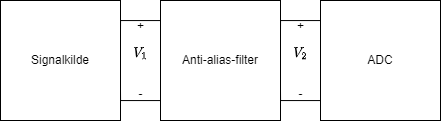
\includegraphics[scale=0.7]{./Images/01Issue/01Anti-alias-filter.png}
	\caption{01Anti-alias-filter.}
	\label{fig:01Anti-alias-filter}
\end{figure}

Dermed skal designes et anti-alias-filter til bruk ved en gitt punktprøvingsfrekvens $f_s$. Filteret skal ha en demping på minst 10 dB ved frekvensen $\frac {f_s} {2}$, og knekkfrekvensen $f_c$ til filteret skal oppfylle $f_c \geq 0.75\frac {f_s} {2}$. Knekkfrekvensen definerer vi som frekvensen hvor amplituderesponsen har sunket med 3 dB fra sitt høyeste nivå.